\setcounter{chapter}{-1}
\chapter{Transformée de Fourier}
\section{Dirac}
\begin{wrapfigure}[15]{r}{4.5cm}
\vspace{-5mm}
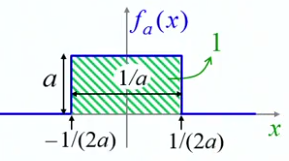
\includegraphics[scale=0.45]{ch1/image1.png}
\captionof{figure}{ }
\end{wrapfigure}
Nous allons commencer par l'étude de la distribution de Dirac, dernier grand 
physicien théoricien du 20$^e$ siècle, notamment en découvrant le positron, 
\dots Ici on va insister sur la \textit{distribution} que l'on peut voir comme 
une généralisation de la notion de fonction. Afin de l'introduire, étudions la 
fonction carrée (ou fenêtre) :


\begin{equation}
f_a(x) =\left\{\begin{array}{ll}
a &\text{ si } |x| \leq \frac{1}{2a}\\
0 &\text{ si } |x| > \frac{1}{2a}
\end{array}\right.
\end{equation}
donnant un rectangle de hauteur $a$ et de largeur $1/a$, sa surface vaut dès lors 
l'unité. 
\begin{equation}
\int_{-\infty}^\infty f_a(x)\ dx = 1
\label{eq:lim1}
\end{equation}
La distribution de Dirac peut être définie à partir de cette fonction 
en prenant la limite de $a$ tendant vers l'infini : sa hauteur tend vers 
l'infini tandis que sa largeur tend vers zéro.
\begin{equation}
\delta(x) = \lim\limits_{a\rightarrow\infty} f_a(x)%pour te simplifier la vie avec les \rightarrow tu peux mettre \to
\end{equation}
On va appeler cette distribution $\delta(x)$ qui représente un pic placé en 
zéro, l'origine est le seul point où l'on trouve une valeur particulière. On 
peut néanmoins dire que la surface sous la courbe vaut l'unité. Cela se 
voit à partir de \autoref{eq:lim1} : la surface sous la courbe ne dépend pas 
du paramètre $a$, d'où la surface unitaire :
\begin{equation}
\int_{-\infty}^\infty \delta(x)\ dx = 1
\end{equation}

\begin{wrapfigure}[7]{l}{4.5cm}
\vspace{-17mm}
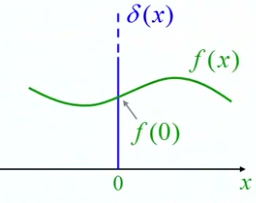
\includegraphics[scale=0.45]{ch1/image2.png}
\captionof{figure}{ }
\end{wrapfigure}
L'intérêt de cette distribution ne se remarque que par combinaison avec d'autres 
fonctions. Considérons le produit d'une fonction quelconque avec la fonction de 
Dirac. La seule valeur qui sera prise en compte est celle qui se trouve en zéro :
\begin{equation}
f(x)\delta(x) = f(0)\delta(x)
\end{equation}
Toutes les valeurs autres que celle de $x$ n'entre pas en ligne de compte. En 
intégrant ce produit 
\begin{equation}
\int_{-\infty}^{\infty} f(x)\delta(x)\ dx = \int_{-\infty}^\infty f(0)\delta(x)\ dx
= f(0)\int_{-\infty}^{\infty}\delta(x)\ dx = f(0)
\end{equation}
On voit cette intégrale comme le "produit-scalaire" de $f$ avec $\delta$ qui 
sélectionne la valeur de la fonction à l'origine. En résumé
\begin{equation}
\delta(x) = \left\{\begin{array}{ll}
\infty & \text{ si } x = 0\\
0 & \text{ si } x \neq 0
\end{array} \right.
\end{equation}

\begin{wrapfigure}[7]{l}{4.5cm}
\vspace{-13mm}
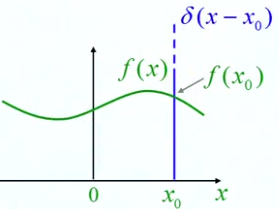
\includegraphics[scale=0.45]{ch1/image3.png}
\captionof{figure}{ }
\end{wrapfigure}
Cette notion peut être généralisée en déplaçant la distribution par translation en 
changeant l'argument $x$ en $x-x_0$ :
\begin{equation}
\delta(x-x_0) = \left\{\begin{array}{ll}
\infty & \text{ si } x=x_0\\
0 & \text{ si } x\neq x_0 
\end{array} \right.
\end{equation}
Cette distribution translatée multipliée par $f$ sélectionnera dès lors la valeur $f(x_0)$. \\

\begin{equation}
\int_{-\infty}^{\infty} f(x)\delta(x-x_0)\ dx = f(x_0)
\end{equation}

La distribution de Dirac peut être définie par une infinité de fonction, tendant 
vers cette fameuse distribution lorsque le paramètre $a$ tend vers zéro. On peut 
par exemple prendre la distribution gaussienne 
\begin{equation}
\delta_a(x) = \frac{1}{a\sqrt{\pi}}e^{-x^2/a^2}  
\end{equation}
Lorsque $a$ tend vers zéro, on obtient un \textit{pic} tendant vers l'infini. On 
peut montrer que cette gaussienne, pour cette limite, tend bien vers la distribution 
de Dirac. Dans le cadre de ce cours, consacré à l'optique de Fourier, la distribution 
intéressante est la suivante
\begin{equation}
\delta_a(x) = \frac{1}{\pi x}\sin\left(\frac{x}{a}\right) = \frac{1}{2\pi}\int_{-1/a}^{1/a}
\cos(kx)\ dk
\end{equation}
Il s'agit d'une définition particulière. La suite du cours justifiera pleinement 
l'utilisation de celle-ci car les transformées de Fourier impliquent les fonction 
harmoniques. On va pouvoir trouver la distribution de Dirac à partir de
\begin{equation}
f(\alpha) = \int_{-\infty}^{\infty} \cos(\alpha x)\ dx
\end{equation}
La résultat dépendra de $\alpha$, ce résultat pourrait bien être une fonction de 
$\alpha$ qui se rapprochera très fortement de la distribution recherchée. Par 
intégration
\begin{equation}
f(\alpha) = \int_{-\infty}^{\infty} \cos(\alpha x)\ dx = \frac{1}{\alpha}\left[
\sin(\alpha x)\right]^\infty_{-\infty} = \frac{1}{a}[\sin(\infty)-\sin(-\infty)]
\end{equation}
Nous sommes face ici à une indétermination, cette intégrale généralisée n'est pas 
directement calculable. Il est préférable de travailler avec la fonction d'intégrale 
de Riemann aux bornes réelles pour ensuite faire tendre celle ci vers l'infini
\begin{equation}
\begin{array}{ll}
f(\alpha) = \int_{-L}^L \cos(\alpha x)\ dx &= \frac{1}{\alpha}[\sin(\alpha L)-\sin(-\alpha 
L)]\\
&= \frac{1}{\alpha}[\sin(\alpha L)+\sin(+\alpha L)]\\
&= 2\frac{\sin(\alpha L)}{\alpha}
\end{array}
\end{equation}

\begin{wrapfigure}[8]{r}{4.5cm}
\vspace{-5mm}
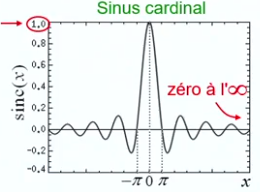
\includegraphics[scale=0.45]{ch1/image4.png}
\captionof{figure}{ }
\end{wrapfigure}
Considérons l'artifice mathématique suivant, permettant de faire apparaître le 
sinus cardinal ($sinc(x) \equiv \sin (x)/x$) :
\begin{equation}
\begin{array}{ll}
f(\alpha) &= 2L \frac{\sin(\alpha L)}{\alpha L}\\
&= 2L\text{sinc}(\alpha L)
\end{array}
\end{equation}
La fonction sinus cardinal tend vers zéro à l'infini, il s'agit d'une fonction paire dont 
la valeur à l'origine vaut l'unité (valeur donnée par la levée de l'indétermination). Cette 
fonction possède des zéros multiples que l'on retrouve à chaque multiple de $\pi$.\newpage

\begin{wrapfigure}[8]{l}{4.5cm}
%\vspace{-5mm}
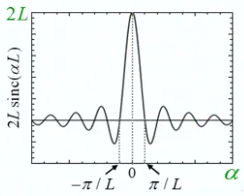
\includegraphics[scale=0.45]{ch1/image5.png}
\captionof{figure}{ }
\end{wrapfigure}
Revenons à nos moutons. Notre fonction sinus cardinal a pour argument $\alpha L$ : les zéros 
de la fonction d'origines se voient tous divisés par $L$ et l'ordonnée à l'origine vaut $2L$. 
Une fois que $\alpha$ n'est plus nul, on redescend brusquement vers un premier zéro (les 
oscillations se comprennent très facilement en interprétant l'aire sous la courbe en faisant 
augmenter $\alpha$).\\
\ \\

\begin{wrapfigure}[8]{r}{7.5cm}
\vspace{-15mm}
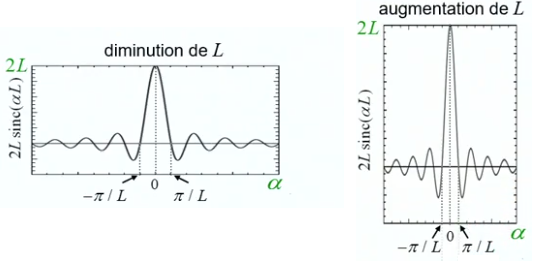
\includegraphics[scale=0.45]{ch1/image6.png}
\captionof{figure}{ }
\end{wrapfigure}
Intéressons nous ce qui se passe lorsque $L \rightarrow \infty$. Remarquons premièrement 
qu'une diminution de $L$ correspond à un \textit{aplatissement} et \textit{élargissent} du 
graphe. Inversement, lorsque $L$ augmente elle gagne en hauteur et les zéros se rapprochent 
de l'origine. Que devient cette fonction pour $L \rightarrow\infty$ ? Montrons que l'on 
obtient, à un facteur près, la distribution de Dirac 
\begin{equation}
f(\alpha) = \lim\limits_{L\rightarrow\infty} \int_{-L}^L \cos(\alpha x)\ dx = \lim\limits_{L 
\rightarrow \infty}[2L\text{sinc}(\alpha L)]
\end{equation}
Cette limite n'est pas facile à appréhender, l'étude du graphe n'est pas fort utile. A 
défaut, on peut s'intéresser à la surface du graphe de cette fonction en étudiant l'aire 
sous la courbe du sinus cardinal :
\begin{equation}
\int_{-\infty}^\infty \text{sinc }(\alpha x)\ dx = \int_{-\infty}^\infty \dfrac{\sin(\alpha
x)}{\alpha x}\ dx = \dfrac{\pi}{\alpha}
\label{eq:AireD}
\end{equation}
\danger Il ne faut pas confondre la variable $\alpha$ avec celle d'intégration, $x$. Nous 
montrons ici que $f(\alpha)$ peut être associée à la distribution. Dans \autoref{eq:AireD} 
remplaçons $x$ par $\alpha$ par "l'ancien $\alpha$" jouera le rôle du paramètre $L$ :
\begin{equation}
\int_{-\infty}^\infty \text{sinc }(L\alpha)\ d\alpha = \int_{-\infty}^\infty \dfrac{\sin(L\alpha)
}{L\alpha}\ d\alpha = \dfrac{\pi}{L}
\end{equation}
En multipliant par $2L$ (pouvant directement rentrer dans l'intégrale):
\begin{equation}
\int_{-\infty}^\infty2L \text{sinc }(L\alpha)\ d\alpha = 2L \int_{-\infty}^\infty \dfrac{\sin(L\alpha)
}{L \alpha}\ d\alpha = 2\pi
\end{equation}
Cette surface vaut $2\pi$, mais ce qui est important est que celui-ci est indépendant 
du paramètre $L$ exactement comme on l'avait pour la fonction fenêtre avec l'aire unitaire ; 
faire tendre $L$ vers l'infini ne change dès lors rien. Les caractéristiques sont celles de 
la fonction de Dirac. Pour retrouver cette distribution, il nous suffit de diviser par $2\pi$.
\begin{equation}
\int_{-\infty}^\infty \lim\limits_{L\rightarrow\infty}[\frac{2L}{2\pi}\text{sinc}(\alpha L)]\ 
d\alpha = \frac{2\pi}{2\pi}=1
\end{equation}
On peut ainsi assimiler ce résultat à la distribution de Dirac :
\begin{equation}
\text{Distribution de Dirac : } \delta(\alpha) = \lim\limits_{L\rightarrow\infty}\left[
\dfrac{L}{\pi}\text{sinc}(\alpha L)\right]
\end{equation}
Cette fonction est \textit{piquée} à l’origine et une largeur tendant vers zéro dont l'aire
sous la courbe vaut bien 1. On peut dès lors écrire
\begin{equation}
f(\alpha) = \lim\limits_{L\rightarrow\infty} \int_{-L}^L \cos(\alpha x)\ dx = \lim\limits_{L 
\rightarrow \infty}[2L\text{sinc}(\alpha L)] = 2\pi \delta(\alpha)
\end{equation}
Sous la forme d'une intégrale généralisée, résultat pratique pour l'étude des transformées 
de Fourier.
\begin{equation}
\int_{-\infty}^\infty \cos(\alpha x)\ dx = 2\pi \delta (\alpha)
\end{equation}
Notons qu'il n'est pas nécessaire de déterminer précisément ce que vaut $\alpha$, la 
"définition" ci-dessous est auto-suffisante
\begin{equation}
\int_{-\infty}^\infty f(\alpha)\delta(\alpha)\ d\alpha = f(0)
\end{equation}
Généralisons \footnote{Il manque l'interprétation en terme d'aire sous le cosinus} quelque
 peu ce que nous venons de faire en vue de passer à la transformée de 
Fourier. La notion de phaseur, exponentielle imaginaire est fondamentale :
\begin{equation}
\int_{-\infty}^\infty e^{i\alpha x}\ dx = \int_{-\infty}^\infty \cos(\alpha x)\ dx + i
\int_{-\infty}^\infty \sin(\alpha x)\ dx
\end{equation}
Cette exponentielle imaginaire cache la fonction $cos(\alpha x)$ que nous venons d'étudier 
avec en plus une partie imaginaire. Que vaut la contribution de la partie imaginaire ? 
\begin{equation}
\int_{-L}^L \sin(\alpha x)\ dx = -\frac{1}{\alpha}\left[\cos(\alpha x)\right]^L_{-L} = 0
\end{equation}
Il n'est même pas ici nécessaire de faire tendre $L\rightarrow\infty$, le cosinus étant 
une fonction paire cela donne tout simplement zéro (directement visible, car l'intégration 
d'une fonction impaire aux bornes centrées sur zéro est identiquement nulle). \\
En conclusion:
\begin{equation}
\dfrac{1}{2\pi}\int_{-\infty}^\infty e^{i\alpha x}\ dx  = \delta(\alpha)
\end{equation}

\newpage
\section{Transformée de Fourier : introduction}
La transformée de Fourier s'applique à une fonction $f(x)$. Pour transformer celle-ci, il 
faut préalablement multiplier par $e^{i\alpha x}$ puis intégration :
\begin{equation}
TF(f) \equiv \int_{-\infty}^\infty f(x)e^{i\alpha x}\ dx = F(\alpha)
\end{equation}
où $F(\alpha)$ est la transformée de Fourier de $f(x)$. Le résultat est bien une fonction 
du paramètre $\alpha$ ! Afin d'illustrer cette définition, reconsidérons le premier exemple 
du chapitre, la fonction fenêtre, cette fois-ci non normalisée.
\begin{equation}
f_a(x) =\left\{\begin{array}{ll}
a &\text{ si } |x| \leq L\\
0 &\text{ si } |x| > L
\end{array}\right.
\end{equation}
Calculons sa transformée de Fourier
\begin{equation}
\begin{array}{ll}
TF(f) &= \int_{-L}^L ae^{i\alpha x}\ dx = a\left[\dfrac{1}{i\alpha}e^{i\alpha x}\right]^L_{-L}\\
&= a\dfrac{1}{i\alpha}\left[e^{i\alpha L}-e^{-i\alpha L}\right] = 2a\dfrac{\sin(\alpha L)}{\alpha}
\end{array}
\end{equation}

\begin{wrapfigure}[8]{l}{4.5cm}
\vspace{-25mm}
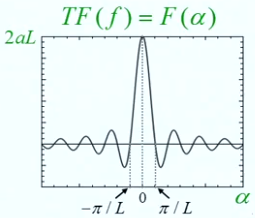
\includegraphics[scale=0.45]{ch1/image7.png}
\captionof{figure}{ }
\end{wrapfigure}
On reconnaît ce que l'on trouvait pour la fonction de Dirac. En multipliant par $L/L$, on obtient 
la transformée de Fourier de la fonction fenêtre
\begin{equation}
TF(f) = 2aL\text{sinc}(\alpha L)
\end{equation}
Il n'y a pour l'instant pas grand chose à comprendre, il ne s'agit que de l'application d'une 
définition. Quel est l'intérêt mathématique de cette transformation? Cette transformation est-elle
réversible ? Oui, c'est son intérêt majeur: la transformée de Fourier inverse.\\
Pour y arriver, étudions la fonction suivante
\begin{equation}
\int_{-\infty}^\infty F(\alpha)e^{-i\alpha x}\ d\alpha  = g(x)
\end{equation}
\danger Il s'agit bien d'un moins, d'où le \textit{inverse}. Le but est de calculer cette intégrale 
pour déterminer notre fameuse inverse dont le résultat sera une fonction de $x$. Remplaçons $F(\alpha)$ 
par son expression (on note $x'$ pour ne pas confondre les variables)
\begin{equation}
g(x)= \int_{-\infty}^\infty \int_{-\infty}^\infty  f(x')e^{i\alpha x'}\ dx'\ e^{-i\alpha x}\ d\alpha
\end{equation}
Par Fubini
\begin{equation}
\begin{array}{ll}
g(x) &= \int_{-\infty}^\infty  f(x') \left(\int_{-\infty}^\infty  e^{i\alpha x'}e^{-i\alpha x}\ d\alpha\right)\ dx'\\
&= \int_{-\infty}^\infty  f(x') \left(\int_{-\infty}^\infty  e^{i\alpha (x'-x)}\ d\alpha\right)\ dx'
\end{array}
\end{equation}
En utilisant une des définition de la distribution de Dirac : $\dfrac{1}{2\pi}\int_{-\infty}^\infty 
e^{i\alpha x}\ dx  = \delta(\alpha)$ en remplaçant $\alpha$ par $x$ et l'ancien $\alpha$ par $L$ :
\begin{equation}
g(x) = \int_{-\infty}^\infty  f(x')\ 2\pi\delta(x'-x)\ dx' = 2\pi f(x)
\end{equation}
Cette intégrale ne sélectionne que la valeur de la fonction $f$ lorsque $x=x'$. 
\begin{equation}
g(x) = \int_{-\infty}^\infty F(\alpha)e^{-i\alpha x}\ d\alpha  = g(x) = 2\pi f(x)
\end{equation}
La \textbf{transformée de Fourier inverse} est donne par
\begin{equation}
TF^{-1}(F) = \frac{1}{2\pi}\int_{-\infty}^\infty F(\alpha)e^{-i\alpha x}\ d\alpha = f(x)
\end{equation}
Petite relation intéressante :
\begin{equation}
TF^{-1}[TF(f)] = f(x)
\end{equation}

\begin{wrapfigure}[6]{l}{5.5cm}
\vspace{-10mm}
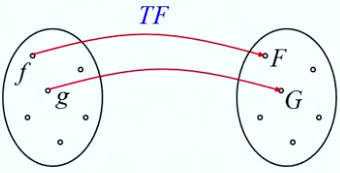
\includegraphics[scale=0.45]{ch1/image8.png}
\captionof{figure}{ }
\end{wrapfigure}
Ceci montre que la transformée de Fourier est une bijection dans l'espace des fonctions. A 
quelques restrictions près, on peut transformer toutes les fonctions par Fourier. Il s'agit 
d'une bijection car deux fonctions distinctes donneront deux transformées différentes, ceci 
vient de l'existence de la transformée inverse. 
\begin{proof}\ \\
\begin{equation}
\begin{array}{ll}
TF(f) = F &\Longrightarrow TF^{-1}[TF(f)] = TF^{-1}[F] = f\\
TF(g) = F &\Longrightarrow TF^{-1}[TF(g)] = TF^{-1}[F] = f = g
\end{array}
\end{equation}
\end{proof}
Il sera dès lors toujours possible de "défaire" une transformée de Fourier de façon univoque. 
Illustrons à nouveau, cette fois-ci avec une gaussienne :
\begin{equation}
f(x) = e^{-x^2/x_0^2}\quad \ft \quad F(\alpha) = x_0\sqrt{\pi}e^{-\alpha^2x_0^2/4}
\end{equation}
Résultat un peu plus compliqué à trouver, il est nécessaire d'utiliser l’analyse complexe. On 
remarque que le résultat est également une gaussienne dont la largeur est inversement 
proportionnelle à $x_0$. Plus la gaussienne est étroite, plus $x_0$ est petit, plus la transformée 
inverse sera large\footnote{Aussi valable pour la fonction fenêtre.}.
Plus la fonction est large, plus sa transformée est étroite et vice-versa la règle est vraiment 
très générale.
\begin{center}
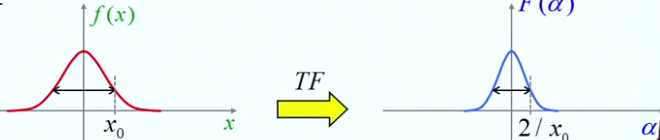
\includegraphics[scale=0.45]{ch1/image9.png}
\captionof{figure}{ }
\end{center}

En faisant tendre $x_0 \rightarrow \infty$ et en supposant une normalisation, on retrouve le delta de 
Dirac $f(x) = \delta(x)$. On peut montrer que si on fait ça, la gaussienne dans le domaine de 
Fourier tend vers l'infini : c'est une constante. Pour trouver la valeur de celle-ci, calculons
\begin{equation}
F(\alpha) = \int_{-\infty}^\infty \delta(x) e^{i\alpha x}\ dx = 1
\end{equation}\\

Considérons un autre exemple : $f(x) = e^{-i\alpha_0x}$. Par application de la définition
\begin{equation}
F(\alpha) = \int_{-\infty}^\infty e^{i(\alpha-\alpha_0)}\ dx = 2\pi\delta(\alpha-\alpha_0)
\end{equation}
\begin{center}
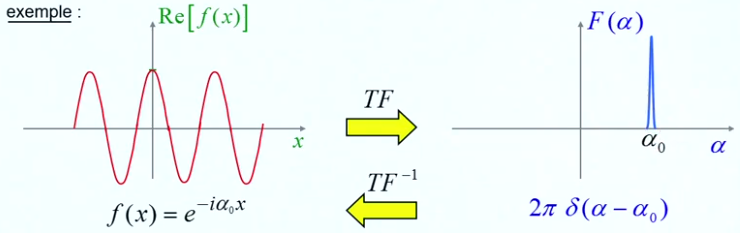
\includegraphics[scale=0.45]{ch1/image10.png}
\captionof{figure}{ }
\end{center}
Le $\alpha_0$ imposant la périodicité de la fonction harmonique localise le "pic" du delta 
de Dirac. La transformée de Fourier de l'exponentielle imaginaire donne directement le delta 
de Dirac. Plutôt que de prendre l'exponentielle je peux faire de même avec le cosinus directement :
\begin{equation}
f(x) = \cos(\alpha_0x) = \frac{e^{i\alpha_0x}+e^{-i\alpha_0x}}{2}
\end{equation}
La seule différence est la contribution de la partie imaginaire
\begin{equation}
F(\alpha) = \int_{-\infty}^\infty f(x)e^{i\alpha x}\ dx = \pi[\delta(\alpha+\alpha_0)+\delta(\alpha
-\alpha_0)]
\end{equation}
\begin{center}
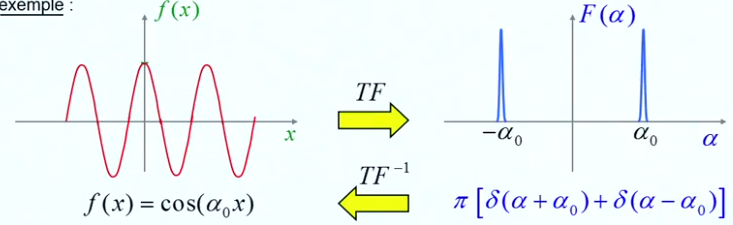
\includegraphics[scale=0.45]{ch1/image11.png}
\captionof{figure}{ }
\end{center}
Dans le cas d'un sinus, il faudra mettre un signe négatif entre les delta et diviser par $i$.\\

Passons en revues les propriétés des transformées de Fourier. Soit la transformée de Fourier
\begin{equation}
F(\alpha) = \int_{-\infty}^\infty f(x)e^{i\alpha x}\ dx
\end{equation}
\begin{equation}
\begin{array}{lll}
\bullet & TF[f(x-x_0)] &= \int_{-\infty}^\infty f(x-x_0)e^{i\alpha x}\ dx\\
&&= \int_{-\infty}^\infty f(x')e^{i\alpha (x'+x_0)}\ dx'\\
&&= e^{i\alpha x_0}\int_{-\infty}^\infty f(x')\ dx'\\
&&= F(\alpha)e^{i\alpha x_0}\ \\
\ \\
\bullet & TF^{-1}[F(\alpha-\alpha_0)] &= f(x)e^{-i\alpha_0 x}\\
\bullet & TF[f(x)e^{-i\alpha_0x}] &= F(\alpha-\alpha_0)
\end{array}
\end{equation}
Ceci peut se résumer avec la fonction de Dirac
\begin{equation}
TF[\delta(x-x_0)] = e^{i\alpha x_0},\qquad TF[e^{-i\alpha_0x}] = \delta(\alpha-\alpha_0)
\end{equation}
Intéressons-nous maintenant à la transformée de Fourier de la dérivée de $f(x)$. Le plus 
simple est d'utiliser la notion de transformée de Fourier inverse
\begin{equation}
f(x) = \frac{1}{2\pi}\int_{-\infty}^\infty F(\alpha)e^{-i\alpha x}\ d\alpha
\end{equation}
En dérivant
\begin{equation}
\begin{array}{ll}
\dfrac{df(x)}{dx} &= \frac{1}{2\pi}\int_{-\infty}^\infty -i\alpha F(\alpha)e^{-i\alpha x}\ 
d\alpha\\
&= TF^{-1}[-i\alpha F(\alpha)]
\end{array}
\end{equation}
On a donc
\begin{equation}
TF\left[\dfrac{df(x)}{dx}\right] = -i\alpha F(\alpha)
\end{equation}
Pour une dérivée seconde, on trouvera $(-i\alpha)^2$, \dots\\

Terminons la section par une généralisation de la transformée de Fourier à deux dimensions. 
Considérons une fonction à deux variables que l'on va multiplier par deux exponentielles de 
sorte à avoir deux variables de Fourier (dites conjuguées, l'une à $x$, l'autre à $y$):
\begin{equation}
F(\alpha,\beta) = \int_{-\infty}^\infty\int_{-\infty}^\infty f(x,y)e^{i\alpha x}e^{i\beta y}\ 
dx\ dy
\end{equation}
A condition de montrer que $f(x,y)$ peut être écrite à partir de la transformée de Fourier 
inverse, on obtient la transformée de Fourier inverse à deux dimensions
\begin{equation}
f(x,y) = \frac{1}{(2\pi)^2} \int_{-\infty}^\infty\int_{-\infty}^\infty F(\alpha,\beta)
e^{-i\alpha x}e^{-i\beta y}\ d\alpha\ d\beta
\end{equation}
Ceci est cohérent et pour s'en rendre compte, substituons l'expression de $F(\alpha,\beta)$ :
\begin{equation}
f(x,y) = \frac{1}{(2\pi)^2} \int_{-\infty}^\infty\int_{-\infty}^\infty \int_{-\infty}^\infty
\int_{-\infty}^\infty f(x',y')e^{i\alpha x'}e^{i\beta y'}\ e^{-i\alpha x}e^{-i\beta y}\
 d\alpha\ d\beta\ dx'\ dy' 
\end{equation}
Par Fubini
\begin{equation}
f(x,y) = \frac{1}{(2\pi)^2} \int_{-\infty}^\infty\int_{-\infty}^\infty f(x',y') \left[\int_{-\infty}^\infty
\left(\int_{-\infty}^\infty e^{i\alpha x'}e^{i\beta y'}\ e^{-i\alpha x}e^{-i\beta y}\
 d\alpha\right)\ d\beta\right]\ dx'\ dy' 
\end{equation}
En intégrant sur $\alpha$
\begin{equation}
f(x,y) = \frac{1}{(2\pi)^2} \int_{-\infty}^\infty\int_{-\infty}^\infty f(x',y') \underbrace{
\int_{-\infty}^\infty e^{i\alpha(x'-x)}\ d\alpha}_{2\pi\delta(x'-x)} \underbrace{\int_{-\infty}^\infty 
e^{i\beta(y'-y)}\ d\beta}_{2\pi\delta(y'-y)}\ dx'\ dy'
\end{equation}
On voit apparaître la distribution de Dirac, de sorte à pouvoir écrire
\begin{equation}
f(x,y) = \int_{-\infty}^\infty\int_{-\infty}^\infty f(x',y')\delta(x'-x)\delta(y'-y)\ dx'\ dy'
\end{equation}
En appliquant la notion de Distribution de Dirac qui "sélectionne" l'argument de la fonction tel 
que l'argument de la fonction de Dirac s'annule c'est-à-dire lorsque $x'=x$ et $y'=y$. Ce résultat-ci 
est bien $f(x,y)$, pas besoin d'aller plus loin. Ceci prouve que le résultat est cohérent.





\newpage
\section{Transformée de Fourier : convolution}
\begin{wrapfigure}[9]{l}{10.5cm}
\vspace{-6mm}
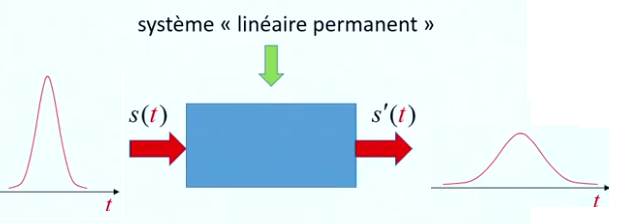
\includegraphics[scale=0.45]{ch1/image12.png}
\captionof{figure}{ }
\end{wrapfigure}
Le théorème de convolution est un théorème fondamental d'un point de vue pratique, il 
justifie l'utilisation de la transformée de Fourier. Considérons un système physique 
linéaire permanent (SLP) dans laquelle rentre un signal $s(t)$ et sort $s'(t)$. Considérons 
que ce SLP soit une fibre optique dans laquelle on peut faire rentrer une impulsion lumineuse. 
Au cours de sa propagation elle va subir des transformation de sorte à avoir une sortie modifiée.
Le système est dit linéaire, il obéit au principe de superposition. Permanent, c'est lorsque 
ce système reste inchangé dans le temps. \\

On peut appliquer le théorème de superposition
\begin{equation}
s(t) = \sum_n s_n(t) \Longrightarrow \text{SLP} \Longrightarrow s'(t) = \sum_n s_n'(t)
\end{equation}

\begin{wrapfigure}[7]{r}{10.5cm}
\vspace{-6mm}
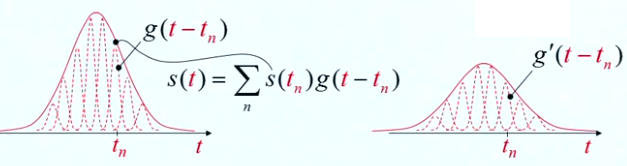
\includegraphics[scale=0.45]{ch1/image13.png}
\captionof{figure}{ }
\end{wrapfigure}
L'idée est de construire une grosse impulsion à partir de la somme d'impulsion plus petite d'amplitude 
progressive pour créer une grosse amplitude gaussienne à partir de la somme de petite gaussienne 
$g(t)$ chacune centrée en $t_n$ donnant lieu à l'enveloppe du signal $s(t)$. Comme on peut le voir, 
l'amplitude d'une gaussienne donne à peu près l'amplitude du champ. Le signal d'entrée peut alors 
être écrit comme étant la somme de toutes ces petites gaussiennes centrées en $t_1,t_2,\dots$ chaque 
fois avec une amplitude qui va donner l'amplitude de l'enveloppe en ce $t_n$\footnote{$s(t_n)$ est 
l'amplitude de la Gaussienne.} :
\begin{equation}
s(t) = \sum_n s(t_n)g(t-t_n)
\end{equation}
A la sortie du SLP, on retrouvera la sortie à chacune des gaussiennes prises séparément.
\begin{equation}
s'(t) = \sum_n s(t_n)g'(t-t_n)
\end{equation}
\danger On retrouve bien $s(t_n)$ et pas $s'(t_n)$ car si l'on place un facteur $a$, par linéarité, 
on retrouvera celui-ci à la sortie.\\

En sommant des gaussiennes, nous n'aurons pas exactement un signal très lisse, il y aura forcément 
des bosses, défauts, \dots Pour représenter des détails arbitrairement fin, on va passer de 
gaussiennes à des distributions de Dirac $g(t-t_n) \rightarrow \delta(t-t_n)$, changeant les 
sommes en intégrales
\begin{equation}
s(t) = \int_{-\infty}^\infty s(t_n)\delta(t-t_n)\ dt_n
\end{equation}
L'amplitude est donnée par $s(t_n)$ et on multiplie par la Dirac en suivant le même raisonnement 
qu'avec des gaussiennes : un continuum de fonction de Dirac
\begin{equation}
s(t) = \int_{-\infty}^\infty s(t')\delta(t-t')\ dt'
\end{equation}
Comment interpréter ça ? En effet, la fonction de Dirac monte jusqu'à l'infini et est arbitrairement 
étroite, ça a du sens ? Oui, le delta de Dirac sélectionne la valeur de la fonction pour laquelle 
celui-ci s'annule, on retrouve bien $s(t)=s(t)$ pour $t'=t$, le raisonnement intuitif suivi ici est bien 
rigoureux. Cette intégrale désigne le \textit{produit de convolution}. On peut alors voir $s(t)$ 
comme sa convolution avec le delta de Dirac. Ceci sera vu en détail plus tard, l'importance est 
de voir ici la cohérence mathématique. En appliquant le principe de superposition on retrouve 
aisément la sortie
\begin{equation}
s'(t) = \int_{-\infty}^\infty s(t')g'(t-t')\ dt'
\end{equation}

Illustrons en considérant que le signal d'entrée est une impulsion de Dirac $s(t) = \delta(t)$, 
il en sortira une certaine réponse $g'(t)$, la \textit{réponse impulsionnelle}, souvent notée $h(t)$. 
La sortie sera alors donnée par la convolution de la réponse impulsionnelle multipliée par le signal 
d'entrée
\begin{equation}
\left\{\begin{array}{ll}
s(t) &= \int_{-\infty}^\infty s(t')\delta(t-t')\ dt'\\
s'(t) &= \int_{-\infty}^\infty s(t')h(t-t')\ dt'
\end{array}\right.
\end{equation}
Une fonction peut vue comme une combili de delta de Dirac multiplié par la fonction elle-même. Cela 
peut paraître trivial mais aussi utile. La sortie sera simplement donnée par la fonction d'entrée 
multipliée par la réponse impulsionnelle ; ce sont les \textit{produits de convolution}.\\

En toute généralité, le système sera entièrement caractérisé par sa réponse impulsionnelle, c'est-à-dire 
si je connais $h(t)$ tout le système est caractérisé ; tout signal d'entrée sera transformé en 
signal de sortie au travers de cette convolution.\\

Hélas le produit de convolution peut être difficile à calculer. Nous allons ici montrer qu'il peut 
être appréhender de façon simple à partir de la notion de transformée de Fourier en introduisant 
les transformations de $s$ et $h$ via la transformation inverse :
\begin{equation}
\left\{\begin{array}{ll}
s(t) &= \frac{1}{2\pi}\int_{-\infty}^\infty S(\omega)e^{-i\omega t}\ d\omega\\
h(t) &= \frac{1}{2\pi}\int_{-\infty}^\infty H(\omega)e^{-i\omega t}\ d\omega
\end{array}\right.
\end{equation}

où $S(\omega)$ est le spectre du signal et $H(\omega)$ est la fonction de transfert spectrale.

En ré-écrivant l'intégrale de convolution (substituer $t$ par $t'$) :
\begin{equation}
\int_{-\infty}^\infty s(t')h(t-t')\ dt' = \int_{-\infty}^\infty \left[\dfrac{1}{2\pi}
\int_{-\infty}^\infty S(\omega)e^{-i\omega t'}\ d\omega\right]h(t-t')\ dt'
\end{equation}
En faisant de même pour $h(t-t')$ (en substituant $t$ par $t-t'$)
\begin{equation}
\int_{-\infty}^\infty s(t')h(t-t')\ dt' = \int_{-\infty}^\infty \left[\dfrac{1}{2\pi}
\int_{-\infty}^\infty S(\omega)e^{-i\omega t'}\ d\omega\right]\left[\frac{1}{2\pi}
\int_{-\infty}^\infty H(\omega')e^{-i\omega'(t-t')}\ d\omega' \right]\ dt'
\end{equation}
En passant à des notations efficaces
\begin{equation}
\int_{-\infty}^\infty s(t')h(t-t')\ dt' = \int_{t'} \left[\dfrac{1}{2\pi}
\int_{\omega} S(\omega)e^{-i\omega t'}\ d\omega\right]\left[\frac{1}{2\pi}
\int_{\omega'} H(\omega')e^{-i\omega'(t-t')}\ d\omega' \right]\ dt'
\end{equation}
Commençons par aborder l'intégrale sur $t'$ (et en sortant le terme en $t$)
\begin{equation}
\int_{-\infty}^\infty s(t')h(t-t')\ dt' = \frac{1}{2\pi}\int_\omega\int_{\omega'}
S(\omega)H(\omega')\ \frac{1}{2\pi}\int_{t'}e^{-i\omega t'}e^{+i\omega't'}\ dt'\ e^{-i
\omega' t}\ d\omega'\ d\omega
\end{equation}
Par propriété des exponentielles
\begin{equation}
\int_{-\infty}^\infty s(t')h(t-t')\ dt' = \frac{1}{2\pi}\int_\omega\int_{\omega'}
S(\omega)H(\omega')\ \underbrace{\frac{1}{2\pi}\int_{t'}e^{-i(\omega-\omega')t'}\ dt'}_{\delta
(\omega-\omega')}\ e^{-i
\omega' t}\ d\omega'\ d\omega
\end{equation}
On retrouve la définition de delta de Dirac grâce au facteur $2\pi$ restant.
\begin{equation}
\int_{-\infty}^\infty s(t')h(t-t')\ dt' = \frac{1}{2\pi}\int_\omega\int_{\omega'}
S(\omega)H(\omega')\ \delta(\omega-\omega')\ e^{-i\omega' t}\ d\omega'\ d\omega
\end{equation}
Effectuons l'intégrale en $\omega'$. Cette intégrale contenant un delta de Dirac, elle 
n'est non nulle qu'en $\omega'=\omega$. 
\begin{equation}
\int_{-\infty}^\infty s(t')h(t-t')\ dt' = \frac{1}{2\pi}\int_\omega
S(\omega)H(\omega)e^{-i\omega t}\ d\omega = TF^{-1}[S(\omega)H(\omega)]
\end{equation}
On reconnaît la transformée de Fourier inverse du produit algébrique de $S$ par $H$.
\begin{equation}
s(t) \otimes h(t) = TF^{-1}[S(\omega)H(\omega)]
\end{equation}
Où encore
\begin{equation}
TF[s(t) \otimes h(t)] = S(\omega)H(\omega)
\end{equation}
C'est le \textbf{théorème de convolution}, fondamental d'un point de vue pratique. En 
effet, plutôt que de devoir effectuer une intégrale contenant un fonction $h$ difficilement 
trouvable on se rapporte à un simple produit dans l'espace de Fourier de la transformée de 
Fourier de la fonction d'entrée par la transformée de Fourier de la fonction de transfert 
qui est bien plus simple à trouver : $H(\omega)$ suffit à caractériser tout le système.\\

\begin{wrapfigure}[11]{r}{10.5cm}
\vspace{-6mm}
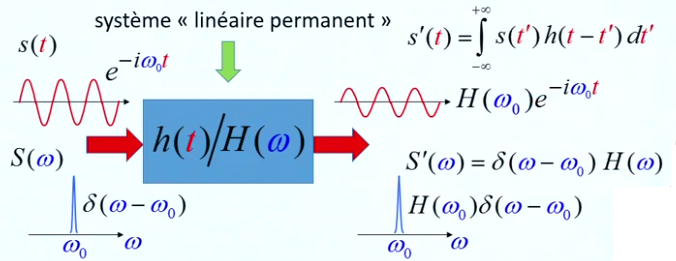
\includegraphics[scale=0.45]{ch1/image14.png}
\captionof{figure}{ }
\end{wrapfigure}
Considérons le delta de Dirac dans le domaine spectral $S(\omega) = \delta(\omega-\omega_0)$. 
La sortie sera donnée par $S'(\omega) = \delta(\omega-\omega_0)H(\omega)$ qui n'est rien 
d'autre que $H(\omega_0)\delta(\omega-\omega_0)$ ! Si l'on repasse dans le domaine temporel, 
on trouve $s(t) = e^{-i\omega_0t}$. A ce signal harmonique correspond une certaine sortie 
donnée par la réponse elle-même donnée par la transformée inverse de $S'(\omega)$, c'est-à-dire 
$H(\omega_0)e^{-i\omega_0t}$. Un système linéaire va conserver le caractère harmonique de 
l'entrée à un facteur près, $H(\omega_0)$.\\

Pour connaître $H(\omega)$, on sait déjà que la fréquence de sortie sera la même : la mesure 
des amplitudes donnera la fonction de transfert. Le système linéaire effectue un transfert 
du signal, une "propagation" entre les deux : un signal harmonique le reste, mais l'amplitude 
se verra être modifiée.\\

En pratique, on ne se contentera pas du domaine temporel. Remontrons la convolution en partant 
depuis l'espace de Fourier pour montrer que ce théorème s'applique aussi pour la transformée 
de Fourier inverse.
\begin{equation}
\left\{\begin{array}{ll}
F(\alpha) &= \int_{-\infty}^\infty f(x)e^{i\alpha x}\ dx\\
G(\alpha) &= \int_{-\infty}^\infty g(x)e^{i\alpha x}\ dx
\end{array}\right.
\end{equation}
Montrons que l'on peut, de façon similaire, écrire
\begin{equation}
H(\alpha) = \int_{-\infty}^\infty f(x)g(x)e^{i\alpha x}\ dx
\end{equation}
Pour se faire, écrivons nos deux fonctions via leurs transformées de Fourier inverse
\begin{equation}
f(x) = \frac{1}{2\pi}\int_{-\infty}^\infty F(\alpha)e^{-i\alpha x}\ d\alpha,\qquad 
g(x) = \frac{1}{2\pi}\int_{-\infty}^\infty G(\alpha)e^{-i\alpha x}\ d\alpha
\end{equation}
En substituant
\begin{equation}
H(\alpha) = \int_x \left[\dfrac{1}{2\pi}\int_{\alpha'} F(\alpha)e^{-i\alpha' x}\ d\alpha'
 \right]\left[\frac{1}{2\pi}\int_{-\alpha''} G(\alpha'')e^{-i\alpha x}\ d\alpha'' \right]
\end{equation}
En commençant par l'intégrale pourtant sur les $x$ afin de refaire apparaître le 
delta de Dirac
\begin{equation}
H(\alpha) = \int_{\alpha'}\int_{\alpha''} F(\alpha')G(\alpha'')\underbrace{\left[\dfrac{1}{2\pi}\int_x 
e^{-i(\alpha'+ \alpha'' -\alpha )x}\ dx\right]}_{\delta(\alpha'+ \alpha'' -\alpha)}\ d\alpha'\ d\alpha''
\end{equation}
En faisant l'intégrale sur $\alpha''$, avec le delta de Dirac il faudra que $\alpha'' = \alpha-\alpha'$. 
On retrouve comme résultat la convolution des deux spectres, des deux transformées de Fourier de 
départ 
\begin{equation}
H(\alpha) = \frac{1}{2\pi}\int_{\alpha'} F(\alpha')G(\alpha-\alpha')\ d\alpha'
\end{equation}

\begin{wrapfigure}[8]{r}{4.5cm}
\vspace{-6mm}
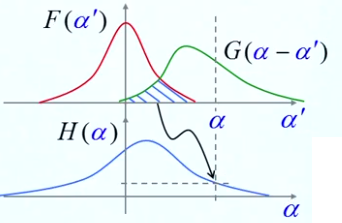
\includegraphics[scale=0.45]{ch1/image15.png}
\captionof{figure}{ }
\end{wrapfigure}
Représentons ces deux variables et faisons le produit. On peut voir ce produit comme un 
recouvrement, les valeurs ne seront non-nulles que la ou elles se recouvrent. Ce recouvrement 
est représenté en bleu ci-contre (vision intuitive). Le résultat de $H(\alpha)$ représente 
ce recouvrement en fonction de $\alpha$ : cette variable représente la \textbf{position} de la
fonction $G$ retournée (car $-\alpha$ en argument). Plus $\alpha$ est proche de $F$, plus 
je me rapproche du recouvrement de mes fonction : c'est ça que représente la convolution ; un 
recouvrement de fonctions dont l'une à été renversée. En conclusion
\begin{equation}
TF[f(x)g(x)] = \frac{1}{2\pi}F(\alpha)\otimes G(\alpha)
\end{equation}














\newpage
\section{La transformée de Fourier : illustration}
Le but de cette section est d'illustrer l'intérêt de cette transformée. On s'intéressera 
ici au cas de la transformée de Fourier temporelle
\begin{equation}
TF(f) = \int_{-\infty}^\infty f(t)e^{i\omega t}\ dt = F(\omega)
\end{equation}
où le $\omega$ est vu comme la pulsation des composantes harmoniques du signal. Par la 
transformée inverse
\begin{equation}
TF^{-1}(F) = \dfrac{1}{2\pi}\int_{-\infty}^\infty F(\omega)e^{-i\omega t }\ d\omega = f(t)
\end{equation}
qui n'est rien d'autre qu'une somme d'onde d'amplitude $F(\omega)$.\\

On se propose d'étudier la propagation d'impulsions lumineuses en fibre optique. On utilisera 
pour ça un laser de fréquence $\omega_0$ extrêmement élevé monochromatique : si c'est le cas, 
la distribution des fréquences sera un delta de Dirac. Décrivons l'onde électromagnétique de 
la façon suivante
\begin{equation}
E(z,t) = ae^{ik(\omega_0)z}e^{-i\omega_0t}
\end{equation}
où $k$, le nombre d'onde, impose la périodicité spatiale. Quand $z$ progresse de $2\pi/k$, on 
progresse bien d'une période. Si l'on ne regarde pas la dépendance temporelle, on retrouve bien 
le phaseur de l'onde à une dimension. Ce qui est important c'est le nombre d'onde
\begin{equation}
k = k(\omega) = \frac{\omega}{c}n(\omega)
\end{equation}
où $n$ est l'indice de réfraction, dépendant de la dynamique des nuages électroniques. Ce $n
(\omega)$ conditionne la propagation en "cachant" toute la complexité microscopique. En pratique, 
il est intéressant de moduler le faisceau laser de sorte à coder des informations. Le champ 
s'en voit dès lors modulée, l'amplitude devient fonction du temps
\begin{equation}
E(0,t) = a(0,t)e^{-i\omega_0t}
\end{equation}
\begin{center}
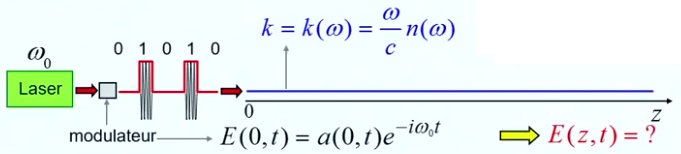
\includegraphics[scale=0.45]{ch2/image1.png}
\captionof{figure}{ }
\end{center}

Ce qui est intéressant est de connaître la sortie du système, que l'on peut considérer comme 
un SLP dont la sortie se trouve en $z$. Introduisons la notion de transformée de Fourier 
temporelle
\begin{equation}
TF(f) = \int_{-\infty}^\infty f(t)e^{i\Omega t}\ dt = F(\Omega)
\end{equation} 
où l'on utilise $\Omega$ car on s'intéresse à la pulsation de l'enveloppe et pas à la 
pulsation rapide $\omega_0$ donnant lieu à cette enveloppe. De même pour la transformée 
inverse
\begin{equation}
TF^{-1}(F) = \dfrac{1}{2\pi}\int_{-\infty}^\infty F(\Omega)e^{-i\Omega t }\ d\omega = f(t)
\end{equation}
Ceci étant fait, on définit le \textbf{spectre} de l'impulsion d'entrée, c'est-à-dire la 
transformée de Fourier suivante
\begin{equation}
A(\Omega) = TF[a(0,t)]
\end{equation}
où
\begin{equation}
a(0,t) = \left\{\begin{array}{ll}
a_0 & \text{ si } |t| \leq T\\
0 & \text{ si } |t| > T
\end{array}\right.\qquad \Rightarrow \quad TF[a(0,t)] = 2a_0T\text{sinc}(\Omega T) = A(\Omega)
\end{equation}
Rappelons qu'une fonction étroite donne une transformée de Fourier large et vice-versa. Nous 
allons maintenant exprimer la fonction comme étant la transformée de Fourier inverse de son 
spectre
\begin{equation}
a(0,t) = TF^{-1}[A(\Omega)]
\end{equation}
Dès lors
\begin{equation}
E(0,t) = \dfrac{1}{2\pi}\int_{-\infty}^\infty A(\Omega)e^{-i\Omega t}\ d\Omega e^{-i\omega_0t}
\end{equation}
En rentrant le facteur exponentiel, il est possible d’interpréter physiquement le résultat
\begin{equation}
E(0,t) = \dfrac{1}{2\pi}\int_{-\infty}^\infty A(\Omega)e^{-i(\omega_0 +\Omega)t}\ d\Omega 
\end{equation}
Le champ à l'entrée de la fibre est donnée par une somme d'onde harmonique dont la pulsation 
n'est plus $\omega_0$ mais $\omega_0+\Omega$ et chacune de ces ondes a une amplitude $A(\Omega)$ 
est donnée par la fonction sinus cardinal qui possède un maximum en $0$.\\

\begin{wrapfigure}[15]{r}{4cm}
\vspace{-5mm}
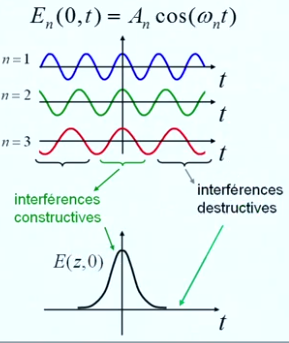
\includegraphics[scale=0.45]{ch2/image2.png}
\captionof{figure}{ }
\end{wrapfigure}
A l'entrée de la fibre, nous retrouvons un \textit{paquet d'onde}. Comment le justifier ? On 
peut intuitivement montré que toute fonction du temps peut être représentée par une 
somme d'onde harmonique (transformée de Fourier inverse). Représentons une somme de cosinus 
d'amplitude différente. A l'origine, les ondes sont en phases sur le maximum. Après un certain 
éloignement, on retrouve des interférences destructives. La combinaison des ondes harmoniques 
peut donner une forme quelconque. Revenons à notre problème physique. 
\begin{equation}
E(0,t) = a(0,t)e^{-i\omega_0t} = \dfrac{1}{2\pi}\int_{-\infty}^\infty A(\Omega)e^{-i(\omega_0
+\Omega)t}\ d\Omega
\end{equation}
La fonction de modulation est donnée par la fonction fenêtre dont nous connaissons la 
transformée de Fourier (sinc). Rappelons qu'une amplitude donnée va bien représenter 
l'amplitude de chacune des ondes harmoniques qui composent le signal. Ceci n'est pas que 
mathématique mais traduit la physique.\\

Notre laser émet des photons à la pulsation $\omega_0$. Ils rentrent dans le modulateur et la 
théorie de Fourier nous dit que oui, la pulsation de l'onde sera changée. Ceci est bien 
physique, il y a réellement une modification de la fréquence du laser\footnote{Ceci se vérifie 
expérimentalement avec un prisme.} $\rightarrow$ l'action du modulateur crée de nouveaux 
photons, une nouvelle distribution d'énergie des photons autour de l'énergie centrale donnée 
par $\hbar\omega_0$. La transformée de Fourier traduit ainsi très bien cette réalité physique.\\

Quel est dès lors le champ pour tout temps, en tout $z$ ? Chaque onde harmonique se propage et 
la façon dont une onde électromagnétique se propage est bien connue : il suffit de rajouter le 
nombre d'onde 
\begin{equation}
E(z,t) =\dfrac{1}{2\pi}\int_{-\infty}^\infty A(\Omega)e^{ik(\omega_0+\Omega)z}e^{-i(\omega_0+\Omega)t}
\ d\Omega
\end{equation}
La seule différence entre cette sortie et l'entrée est un facteur exponentiel correspondant, 
comme vu précédemment, à la \textbf{fonction de transfert} du système. Or, la fonction $k(
\omega_0+\Omega)$ est connu, la fonction de transfert, le \textit{propagateur} est connu. Pour 
tout $z$ on introduit la fonction de transfert qui est un simple facteur de phase qui est connu 
car l'indice de réfraction de la fibre est connue. Simplifions l'expression par son approximation 
au premier ordre
\begin{equation}
k(\omega_0+\Omega) \approx k(\omega_0)+k'(\omega_0)\Omega+\dots\qquad \left(k'=\dfrac{dk}{d\omega}
\right)
\end{equation}
Par substitution
\begin{equation}
E(z,t) =\dfrac{1}{2\pi}\int_{-\infty}^\infty  A(\Omega)e^{i(k_0+k_0'\Omega)z}e^{-i(\omega_0+
\Omega)t}
\ d\Omega
\end{equation}
Sortons tout ce qui ne dépend pas de $\Omega$
\begin{equation}
E(z,t) =\dfrac{1}{2\pi}\int_{-\infty}^\infty  A(\Omega)e^{ik_0'\Omega z}e^{-i\Omega t}\ d\Omega\ \ 
e^{ik_0 z}\ e^{-i\omega_0 t}
\end{equation}
Regroupons les exponentielles
\begin{equation}
E(z,t) =\underbrace{\dfrac{1}{2\pi}\int_{-\infty}^\infty  A(\Omega)e^{i\Omega(t-k_0'z)}\ d\Omega}_{
a(0,t-k_0'z)}\ \ 
e^{ik_0 z}\ e^{-i\omega_0 t}
\end{equation}

\begin{wrapfigure}[7]{l}{6cm}
\vspace{-5mm}
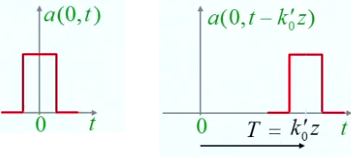
\includegraphics[scale=0.45]{ch2/image3.png}
\captionof{figure}{ }
\end{wrapfigure}
Cette expression n'est que la transformée de Fourier inverse du spectre du modulateur à laquelle 
on rajoute le propagateur de chacune des ondes harmoniques. Dès lors, en "oubliant" le $k_0'z$ 
on reconnaît la transformée inverse. La seule différence avec le signal de départ est une 
translation temporelle de $k_0'z$.
\begin{equation}
E(z,t) = a(0,t-k_0'z)e^{ik_0z}e^{-i\omega_0t}
\end{equation}
En sortie, on retrouvera en $z$ le signal ci-dessus. Ce n'est rien d'autre que le signal d'entrée 
translaté de $k_0'z$. Que représente cette translation? Il se cache la dedans la notion de 
vitesse de groupe. Si le temps $k_0'z$, l'impulsion s'est déplacée de $z$. On peut faire 
apparaître la notion de vitesse de groupe
\begin{equation}
v_g = \dfrac{z}{T} = \dfrac{1}{k_0'} = \left.\dfrac{dk}{d\omega}\right|_{\omega_0}^{-1}
\end{equation}
où $T = k_0'z$ est le temps de propagation. Ce résultat est obtenu par approche au premier 
ordre. Un développement au second ordre mettrait en évidence le phénomène de dispersion.























